\chapter{Requisitos de Software}

\section{Requisitos Funcionais}

\subsection{RF1: Iniciar programa}\label{subsection:RF1}
Ao iniciar, o programa deve mostrar uma janela de \textit{pop-up} com um único campo, solicitando que o jogador informe
o seu nome. Após o recebimento desta informação, fechar o \textit{pop-up} e mostrar a janela principal do jogo.
A interface deverá mostrar o \hyperref[fig:configuracao tabuleiro]{tabuleiro em sua configuração inicial} e um botão que
de ``Iniciar Jogo''. Ao solicitar \rfreference{RF2}{Iniciar jogo}, o programa deverá requisitar uma conexão com o servidor;
\begin{itemize}
  \item Caso a conexão seja bem sucedida, apresentar uma mensagem de sucesso ao usuário e liberar demais funcionalidades do jogo;
  \item Caso contrário, informar o erro ao usuário e apresentar as opções:
    \begin{itemize}
        \item Tentar novamente;
        \item Fechar o programa;
    \end{itemize}
\end{itemize}

\subsection{RF2: Iniciar jogo}\label{subsection:RF2}
Na interface inicial apresentada ao \rfreference{RF1}{Iniciar programa}, está inclusa a ação ``\textbf{Iniciar jogo}"",
liberada após o jogador informar seu nome. Para iniciar a partida, o programa enviará uma requisição ao servidor, que
caso bem-sucedida, mostrará qual jogador realizará a primeira jogada, assim como suas respectivas identificações.
\subparagraph{} A interface deverá ser atualizada com as informações recebidas; caso o jogador local seja quem inicia a
partida, a interface deve estar habilitada para seu procedimento de lance \rfreference{RF4}{Selecionar peça}. Esta
funcionalidade só deve estar habilitada se o programa estiver em seu estado inicial, isto é, sem partida em andamento e
com o tabuleiro em seu estado inicial. 

\subsection{RF3: Restaurar estado inicial}\label{subsection:RF3}
O programa deve apresentar a opção de menu ``\textbf{Restaurar estado inicial}'' para reverter o programa à sua
configuração inicial, isto é, sem partida em andamento e com o \hyperref[fig:configuracao tabuleiro]{tabuleiro em seu
estado inicial}. Esta funcionalidade só deve estar habilitada se o programa estiver com uma partida finalizada.

\subsection{RF4: Selecionar peça}\label{subsection:RF4}
O programa deve permitir a um jogador, quando está em seu turno, selecionar uma de suas peças no tabuleiro para jogar.
\begin{itemize}
  \item Caso o oponente tenha realizado um lance que configura uma \textit{vitória} no final do tabuleiro, e esta for
    \textit{contestável} (ver \hyperref[section:regras]{Regras do jogo}), então o jogador deve, obrigatoriamente,
    selecionar uma das peças que contestará a vitória do oponente;
  \item Caso contrário, o jogador pode selecionar qualquer uma de suas peças que possam realizar movimentos
    imediatamente;
\end{itemize}
As peças passíveis de seleção devem ser destacadas na interface. A peça selecionada deve, também, visualmente destacada
da interface do programa, e após a seleção a interface deve destacar visualmente as posições para qual a peça pode ser
movida; caso uma ou mais posições alcançáveis configure uma \textit{captura} de uma peça do oponente, esta posição
deve distinguir-se visualmente das demais alternativas, sinalizando que representa uma \textit{captura}, e não apenas um
movimento.

\subsection{RF5: Selecionar destino} \label{subsection:RF5}
O programa deve permitirá que um jogador, após realizar \rfreference{RF4}{Selecionar peça}, selecione a posição de
destino desta mesma peça, de acordo com o tipo de movimentos dessa peça, da configuração atual do tabuleiro, e do atual
estado da partida (ver \hyperref[section:regras]{Regras do jogo});
\begin{itemize}
  \item Caso exista uma peça do oponente em uma \hyperref[section:progressao]{posição que exige ser contestada}, esta
    posição deverá ser a única passível de seleção, e deverá ser visualmente realçada para sinalizar que pode ser
    selecionada;
  \item Caso contrário, todas as possíveis posições alcançáveis pela peça em sua posição atual devem ser destacadas e
    habilitadas para seleção;
\end{itemize}
Ao realizar a seleção de uma posição válida para completar o movimento, a instância do programa deve enviar ao servidor
uma mensagem contendo informações sobre a jogada:

\begin{description}
  \item[Peça selecionada:] Um identificador que especifique qual peça está sendo movimentada no lance;
  \item[Posição de origem:] Posição de origem do movimento;
  \item[Posição de destino:] Posição de destino do movimento;
  \item[Estado da partida:] Estado da partida, determinado pela última jogada; pode ser um valor entre:
    \begin{description}
      \item[EM ANDAMENTO:] Quando o movimento realizada não categoriza, imediatamente, uma vitória para o jogador que
        realizou a jogada;
      \item[FINALIZADA:] Quando o movimento categoriza, precisamente, uma \textit{vitória} para o jogador que realiza a
        jogada (ver \hyperref[section:progressao]{Progressão da partida});
    \end{description}
\end{description}
Caso um movimente categorize uma \textit{vitória} e finalize a partida, apresentar ao usuário a opção de
\rfreference{RF3}{Restaurar estado inicial}.

\subsection{RF6: Receber determinação de início} \label{subsection:RF6} 
O programa deve receber e processar uma notificação de início de partida, originada no servidor, em função de 
solicitação de início de partida por parte de outro jogador conectado ao servidor. O procedimento a partir do 
recebimento da notificação de início é o mesmo descrito no \rfreference{RF2}{Iniciar jogo}, isto é, a interface do 
programa deve ser atualizada com as informações recebidas. Caso o jogador local seja quem inicia a partida, a interface 
deve estar habilitada para seu procedimento de lance, especificado em \rfreference{RF4}{Selecionar peça} e
\rfreference{RF5}{Selecionar destino}.

\subsection{RF7: Receber jogada} \label{subsection:RF7} 
O programa deve poder receber e processar uma jogada do adversário, enviada pelo servidor, quando for o turno do oponente
jogar. A jogada recebida deve ser um lance regular e conter as informações especificadas para o envio de jogada no 
\rfreference{RF5}{Selecionar destino}. O programa deve remover a peça de origem definida e colocá-la no destino, e 
atender os critérios a seguir:

\begin{itemize}
  \item O programa deve processar uma \textit{captura}, quando este for o cenário caracterizado pela jogada recebida, 
    removendo a peça capturada do tabuleiro;
  \item O programa deve processar uma \textit{vitória} do oponente, quandoo este for o cenário caracterizado pela jogada
    recebida, finalizando a partida e apresentando \rfreference{RF3}{Restaurar estado inicial}, da mesma forma como
    acontece em \rfreference{RF5}{Selecionar destino};
  \item O programa deve processar uma situação de \textit{contestação obrigatóra}, quando este for o cenário
    caracterizado pela jogada recebida, obrigando o jogador local a contestar o último lance do oponente, como
    especificado em \rfreference{RF4}{Selecionar peça} e \rfreference{RF5}{Selecionar destino};
\end{itemize}
Caso a jogada não caracterize nenhum dos casos especiais listados acima, o programa segue para o turno do jogador local,
com \rfreference{RF4}{Selecionar peça}.

\subsection{RF8: Receber notificação de abandono} \label{subsection:RF8} 
O programa deverá poder receber e processar um sinal de abandono de partida por parte do oponente remoto, enviada pelo
servidor; neste caso, a partida deve ser considerada encerrada e o abandono notificado na interface, apresentando ao 
usuário a opção de \rfreference{RF3}{Restaurar estado inicial}.

\section{Requisitos Não-Funcionais}

\subsection{RNF1: Tecnologia de interface gráfica para usuário} \label{subsection:RNF1}
A interface gráfica deve ser baseada em \gls{tkinter}.

\subsection{RNF2: Suporte para a especificação de projeto} \label{subsection:RNF2}
A especificação e documentação do projeto deve ser produzida com a ferramenta \gls{visualparadigm}.

\subsection{RNF3: Interface do programa} \label{subsection:RNF3}
A interface do programa será produzida conforme o esboço da imagem abaixo:

\begin{figure}[h]
    \centering
    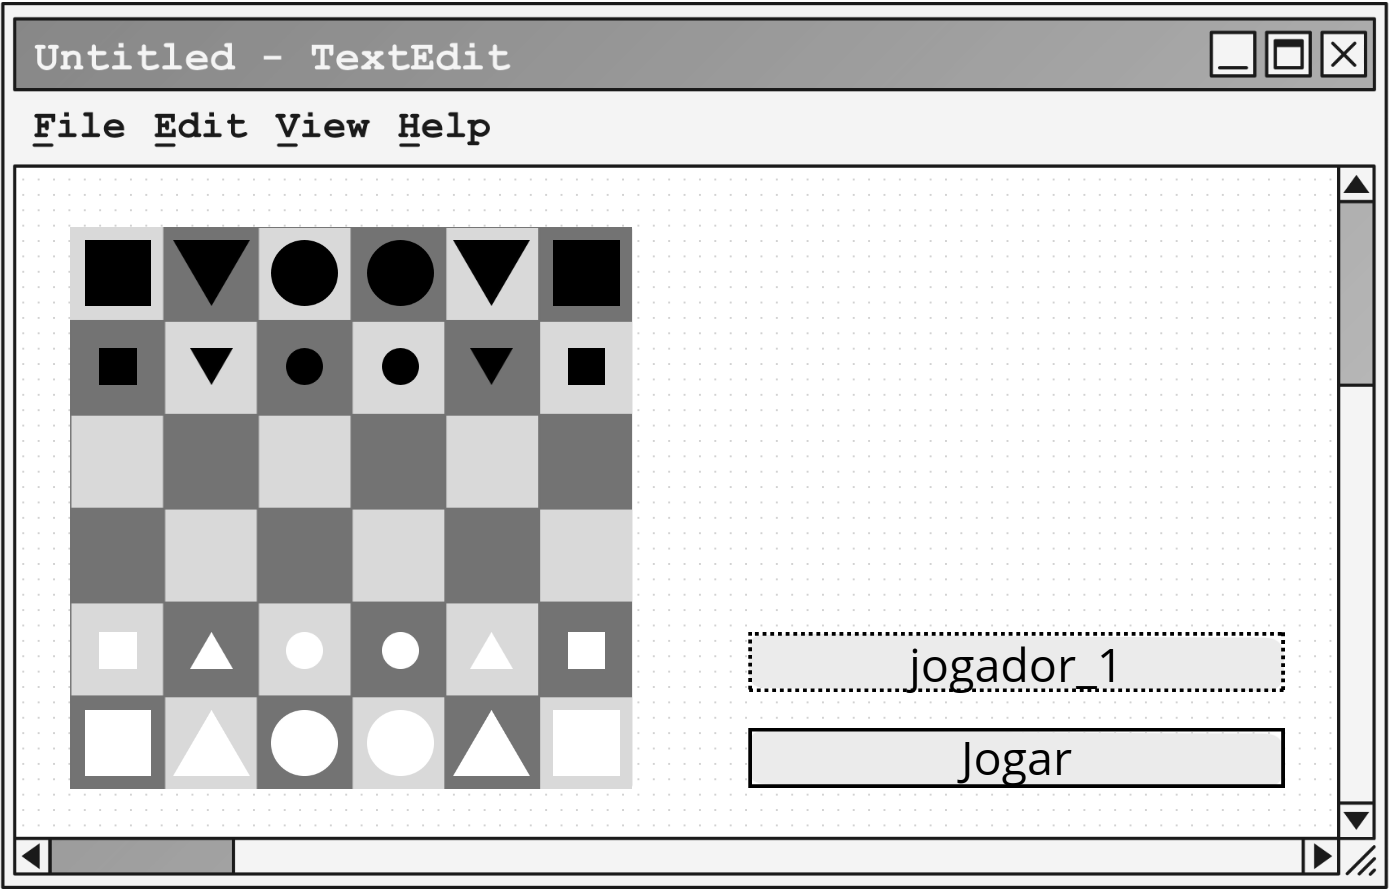
\includegraphics[width=15cm]{Images/figure_2_graphical_interface}
    \caption{\textit{Mockup} de interface gráfica do programa}
    \label{fig:interface tabuleiro}
\end{figure}

